%20 min preso!
\documentclass[xcolor=table]{beamer}
\usepackage{beamerthemesplit}
\usepackage{wrapfig}
\usetheme{SPbGU}
\usepackage{pdfpages}
\usepackage{amsmath}
\usepackage{cmap}
\usepackage[T2A]{fontenc}
\usepackage[utf8]{inputenc}
\usepackage[english]{babel}
\usepackage{indentfirst}
\usepackage{amsmath}
\usepackage{tikz}
\usepackage{multirow}
\usepackage[noend]{algpseudocode}
\usepackage{algorithm}
\usepackage{algorithmicx}
\usepackage{fancyvrb}
\usetikzlibrary{calc}
\usetikzlibrary{shapes,arrows}
\usetikzlibrary{arrows,automata}
\usetikzlibrary{positioning}

\usepackage{minted}
\usepackage{verbments}

\usepackage{tabularx}
\newcolumntype{Y}{>{\raggedleft\arraybackslash}X}


\newtheorem{mytheorem}{Theorem}
\renewcommand{\thealgorithm}{}

\newcommand{\tikzmark}[1]{\tikz[overlay,remember picture] \node (#1) {};}
\def\Put(#1,#2)#3{\leavevmode\makebox(0,0){\put(#1,#2){#3}}}

\tikzset{
    state/.style={
           rectangle,
           rounded corners,
           draw=black, very thick,
           minimum height=2em,
           inner sep=2pt,
           text centered,
           },
}

\beamertemplatenavigationsymbolsempty

\title[Bar-Hillel Theorem in Coq]{Bar-Hillel Theorem Mechanization in Coq}
%\subtitle[YaccConstructor]{Parsing techniques for graph analysis}
% То, что в квадратных скобках, отображается в левом нижнем углу.
\institute[JetBrains Research]{
JetBrains Research, Programming Languages and Tools Lab  \\
Saint Petersburg University
}

% То, что в квадратных скобках, отображается в левом нижнем углу.
\author[Semyon Grigorev]{Sergey Bozhko, Leyla Khatbullina, \textbf{Semyon Grigorev}}

\date{July 05, 2019}

\begin{document}
{
\begin{frame}[fragile]
  \begin{table}
  \centering
  \begin{tabularx}{\linewidth}{YcX}
    
\includegraphics[height=1.5cm]{pictures/jetbrainsResearch.pdf} \hfill
    & \begin{minipage}[t]{0.3\textwidth}\center \vspace{-1cm}  WoLLIC 2019
      \end{minipage}
    & \hfill 
\includegraphics[height=1.5cm]{pictures/SPbGU_Logo.png}
  \end{tabularx}
  \end{table}
  \titlepage
\end{frame}
}

\begin{frame} \frametitle{Automated Theorem Proving}
  \begin{itemize}
    \item Yet another attemt to automate proof correctness checking
    \item In some systems --- a way to create correct by construction algorithms
    \begin{itemize}
      \item Coq
    \end{itemize}

  \end{itemize}

\end{frame}


\begin{frame} \frametitle{Formal Language Theory Mechanization}

\begin{itemize}
  \item Nontrivial proofs checking
  \item Correctness of algorithms
\end{itemize}

\end{frame}

\begin{frame} \frametitle{The Bar-Hillel Theorem}
\begin{theorem}[Bar-Hillel]
	If $L_1$ is a context-free language and $L_2$ is a regular language, then $L_1 \cap L_2$ is context-free.
\end{theorem}
\end{frame}

\begin{frame} \frametitle{Context-Free Path Quierying (CFPQ)}
  \begin{minipage}[m]{0.45\linewidth}
  \onslide<1-6>{Navigation through a edge-labelled graph}

  \begin{itemize}
    \onslide<3-6>{
    \item Whether exist paths in graph, such that they looks like well-balanced sequences over \texttt{A} and \texttt{B}?
    }
    \onslide<4-6>{
    \item Find all paths, such that thay form a world in the Dyck language over \texttt{A} and \texttt{B}
    }
  \end{itemize}

  \end{minipage}
  \hfill
  \begin{minipage}[m]{0.5\linewidth}
  \onslide<2-6>{
  \begin{figure}
        \begin{tikzpicture}[shorten >=1pt,node distance=2cm,on grid,auto]
   \node[state] (q_1)   {$1$};
   \node[state] (q_2) [above=of q_1] {$2$};
   \node[state] (q_3) [above right=of q_1, below right=of q_2] {$0$};
   \node[state] (q_4) [right=of q_3] {$3$};
    \path[->]
    (q_1) edge  node {A} (q_2)
    (q_2) edge  node {A} (q_3)
    (q_3) edge  node {A} (q_1)
    (q_3) edge[bend left, above]  node {B} (q_4)
    (q_4) edge[bend left, below]  node {B} (q_3);
\end{tikzpicture}
\end{figure}
  }
  \vspace{0.5cm}
  \onslide<5-6>{
  Paths filter (query):
  $$s \to A \ s \ B \ s \mid \varepsilon$$
  }
  \end{minipage}
  \vspace{0.2cm}
\onslide<6>{
Answer:
\begin{itemize}
  \item $2 \xrightarrow{A} 0 \xrightarrow{B} 3$
  \item $1 \xrightarrow{A} 2 \xrightarrow{A} 0 \xrightarrow{B} 3 \xrightarrow{B} 0$
  \item $\ldots$
\end{itemize}
}
\end{frame}


\begin{frame} \frametitle{CFPQ: Formal View}
  \begin{itemize}
    \item $\mathbb{G} = (\Sigma, N, P, S)$ --- context-free grammar
    \begin{itemize}
    %  \item $A \rightarrow B C$, where $A, B, C \in N$
   %   \item $A \rightarrow x$, where $A \in N, x \in \Sigma$
      \item $L(\mathbb{G}) = \{ w \mid S \Rightarrow^* w \}$
    \end{itemize}
    \pause
    \item $G = (V,E,L)$ --- directed graph
      \begin{itemize}
        \item $v \xrightarrow{l} u \in E$
        \item $L \subseteq \Sigma$
      \end{itemize}
      \pause
    %\item $p = v_0 \xrightarrow{l_0} v_1 \xrightarrow{l_1} \cdots \xrightarrow{l_{n-2}} v_{n-1} \xrightarrow{l_{n-1}} v_n$ --- path in $G$
    \item $\omega(\pi) = \omega(v_0 \xrightarrow{l_0} v_1 \xrightarrow{l_1} \cdots \xrightarrow{l_{n-2}} v_{n-1} \xrightarrow{l_{n-1}} v_n) = l_0 l_1 \cdots l_{n-1}$
    \pause
    \item $R = \{ (n, m) \mid \exists n \pi m$, such that $\omega(\pi) \in L(\mathbb{G})\}$
    \pause
    \item $P = \{ \pi \mid \pi$ is a path in $G$, such that $\omega(\pi) \in L(\mathbb{G})\}$
  \end{itemize}
\end{frame}


\begin{frame} \frametitle{Applications of CFPQ}
\begin{itemize}
	\item Graph data base querying
  \begin{itemize}
  	\item Yannacacis !!!
    \item Static code analysis
  \end{itemize}
  \pause
  \item Static code analysis
  \begin{itemize}
  	\item Reps !!!
    \item Static code analysis
  \end{itemize}
\end{itemize}
\end{frame}


\begin{frame} \frametitle{Sketch of the Proof}
\begin{enumerate}
  \item Assume that there is a contextfree grammar $\mathbb{G}_{CNF}$ in Chomsky normal form, such that $L(\mathbb{G}_{CNF}) = L_1$
  \pause
  \item Assume that there is a set of regular languages $\{A_1 \ldots A_n\}$ where each $A_i$ is recognized by a DFA with precisely one final state and $L_2 = A_1 \cup \ldots \cup A_n$
  \pause
  \begin{itemize}
    \item If $ L \neq \varnothing $ and $L$ is regular then $L$ is the union of regular language $A_1, \ldots , A_n$ where each $A_i$ is accepted by a DFA with exactly one final state
  \end{itemize}
  \pause
  \item For each $A_i$ we can explicitly define a grammar of the intersection: $L(\mathbb{G}_{CNF}) \cap A_i$
  \pause
  \item Finally, join them together with the operation of the union
\end{enumerate}

\end{frame}

\begin{frame}[fragile] \frametitle{Hofmann's Results Generalization}

Jana Hofmann provides mechanization of the part of CFL in the Coq
\begin{itemize}
    \item Basic definitions: terminal, nonterminal, grammar, word, $\dots$
    \pause
    \item \textbf{Context-Free grammar to the Chomsky Normal Form convertion}
\end{itemize}
\pause

\begin{center}
  \begin{minipage}[t]{0.47\textwidth}
\begin{center}
    \begin{pyglist}[language=coq, numbers=none, numbersep=5pt]
    Inductive ter : Type :=
     | T : nat -> ter.
  	\end{pyglist}

    Jana Hofmann
  \end{center}
  \end{minipage}
  \pause
  ~ \vline \vline ~
  \begin{minipage}[t]{0.47\textwidth}
\begin{center}
    \begin{pyglist}[language=coq, numbers=none, numbersep=5pt]
    Inductive ter : Type :=
     | T : Tt -> ter.
    \end{pyglist}

    We need an arbitrary type for terminals and nontermianls!
  \end{center}
  \end{minipage}

\pause
\vspace{0.5cm}
And now we should carefully rewrite all existing stuff \dots
\end{center}


\end{frame}


\begin{frame}[fragile] \frametitle{DFA Splitting}
If $ L \neq \varnothing $ and $L$ is regular then $L$ is the union of regular language $A_1, \ldots , A_n$ where each $A_i$ is accepted by a DFA with precisely one final state
\pause
\begin{pyglist}[language=coq, numbers=none, numbersep=5pt]
Lemma correct_split:
   forall dfa w,
     dfa_language dfa w <->
     exists sdfa,
        In sdfa (split_dfa dfa) /\ s_dfa_language sdfa w.
\end{pyglist}
\end{frame}

\begin{frame}[fragile] \frametitle{Chomsky Induction}

  \begin{lemma} \label{lemma:chomskyind1}
  Let $\mathbb{G}$ be a grammar in CNF. Consider an arbitrary nonterminal $N \in \mathbb{G}$ and phrase which consists only of terminals $w$.
  If $w$ is derivable from $N$ and $|w| \ge 2$, then there exists two nonterminals $N_1, N_2$ and two phrases $w_1, w_2$ such that: $N \to N_1 N_2 \in \mathbb{G}$, $der(\mathbb{G}, N_1, w_1)$, $der(\mathbb{G}, N_2, w_2)$, $|w_1| \ge 1$, $|w_2| \ge 1$ and $w_1 \mathbin{++} w_2 = w$.
  \pause
  \end{lemma}
\begin{center}
  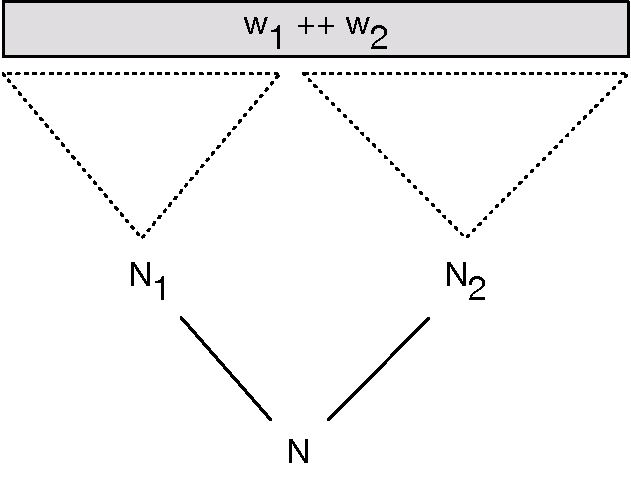
\includegraphics[height=4.5cm]{pictures/ChomskyInductionIntuition.pdf}
\end{center}
\end{frame}

\begin{frame}[fragile] \frametitle{Chomsky Induction in Coq}

\begin{pyglist}[language=coq, numbers=none, numbersep=5pt]
Definition syntactic_analysis_is_possible :=
forall (G : grammar) (A : var) (w : phrase),
   der G A w -> (R A w \in G)
                \/
                (exists rhs, R A rhs \in G /\ derf G rhs w).

\end{pyglist}
\end{frame}

\begin{frame}[fragile] \frametitle{Languges Union}

  \begin{pyglist}[language=coq, numbers=none, numbersep=5pt]
  Variable grammars: seq (var * grammar).

  Theorem correct_union:
  forall word,
    language (grammar_union grammars) (V (start Vt))
             (to_phrase word)
    <->
    exists s_l,
      language (snd s_l) (fst s_l) (to_phrase word)
      /\
      In s_l grammars.
  \end{pyglist}

\end{frame}



\begin{frame}[fragile] \frametitle{The Final Theorem}

\begin{theorem}
    For any two decidable types $\textbf{Tt}$ and $\textbf{Nt}$ for types of terminals and nonterminals correspondingly. If there exists a bijection from $\textbf{Nt}$ to $\mathbb{N}$ and syntactic analysis is possible (in the sense of our definition), then for any DFA \textbf{\textit{dfa}} and any context-free grammar $\mathbb{G}$, there exists the context-free grammar $\mathbb{G}_{INT}$, such that $L(\mathbb{G}_{INT}) = L(\mathbb{G}) \cap L(\textit{dfa})$.
\end{theorem}

\end{frame}

\begin{frame}[fragile] \frametitle{The Final Theorem in Coq}

  %\begin{listing}[h]
      \begin{pyglist}[language=coq, numbers=none, numbersep=5pt]

  Theorem grammar_of_intersection_exists:
    exists
     (NewNonterminal: Type)
     (IntersectionGrammar: @grammar Terminal NewNonterminal)
     St,
    forall word,
      dfa_language dfa word /\ language G S (to_phrase word)
      <->
      language IntersectionGrammar St (to_phrase word).
     \end{pyglist}
  %\caption{Final theorem}
  %\label{lst:lang-eq}
  %\end{listing}

\end{frame}

\begin{frame} \frametitle{Conclusion}

\begin{itemize}
 \item We present mechanized in Coq proof of the Bar-Hillel theorem on the closure of context-free languages under intersection with the regular languages
 \item We generalize the results of Jana Hofmann and Gert Smolka
 \begin{itemize}
   \item The definition of the terminal and nonterminal alphabets in context-free grammar were made generic
   \item All related definitions and theorems were adjusted to work with the updated definition

 \end{itemize}

 \item All results are published at GitHub and are equipped with automatically generated documentation

\end{itemize}

\end{frame}

\begin{frame} \frametitle{Future work}

\begin{itemize}
 \item Ruy J. G. B. de Queiroz vs Jana Hifmann
 \begin{itemize}
   \item We use results of Jana Hofman
   \item Results of Ruy J. G. B. de Queiroz looks more mature
   \item Is it possible to create one ``true'' solution in this area?
   \begin{itemize}
     \item Wether our grammar-based proof is always better then PDA-based one?
   \end{itemize}
 \end{itemize}
 \pause
 \item Mechanization of practical algorithms which are just implementation of the Bar-Hillel theorem
 \begin{itemize}
   \item Context-free path querying algorithm, based on CYK or even on GLL parsing algorithm
   \item Certified algorithm for context-free constrained path querying for graph databases
 \end{itemize}
\end{itemize}

\end{frame}



\begin{frame}
\frametitle{Contact Information}
\begin{itemize}
  \item Semyon Grigorev:
    \begin{itemize}
      \item \href{mailto:s.v.grigoriev@spbu.ru}{s.v.grigoriev@spbu.ru}
      \item \href{mailto:Semen.Grigorev@jetbrains.com}{Semen.Grigorev@jetbrains.com}
    \end{itemize}
  \item Sergey Bozhko:
  \begin{itemize}
    \item  Max Planck Institute for Software Systems (MPI-SWS), Saarbrcken, Germany
    \item  \href{mailto:sbozhko@mpi-sws.com}{sbozhko@mpi-sws.com}
  \end{itemize}
    \item Leyla Khatbullina:
  \begin{itemize}
    \item St.Petersburg Electrotechnical University ``LETI'', St.Petersburg, Russia
    \item  \href{mailto:leila.xr@gmail.com}{leila.xr@gmail.com}
  \end{itemize}
  \item Sources: \href{https://github.com/YaccConstructor/YC_in_Coq}{https://github.com/YaccConstructor/YC\_in\_Coq}
\end{itemize}
\vspace{0.5cm}
\center{\huge{Thanks!}}
\end{frame}
\end{document}
